\documentclass[12pt,a4]{article}
\pagestyle{plain}                           

% Use Report Template
\usepackage{report_template}

% For appendix
\usepackage[toc,page]{appendix}

\usepackage{tabularx}

% For Fortran Code
\usepackage{listings}
\lstset{language=[90]Fortran,
  basicstyle=\ttfamily,
  keywordstyle=\bfseries,
  commentstyle=\itshape,
  morecomment=[l]{!\ },% Comment with only space after !
  showstringspaces=false,
  frame=topline
}

% Indent
\setlength\parindent{1 in}

\begin{document}
\title{Naive Tsunami Generation via Shallow Water Theory\\
\large  MATH484 Final Project Report}
\author{John Luke Lusty, Jonah Kopp, Clay Kramp, Lonny Cox-Lauf}
\date{April 12\textsuperscript{th}, 2018}

\begin{titlepage}
	\maketitle
    \begin{figure}[h]
        \centering
        \fbox{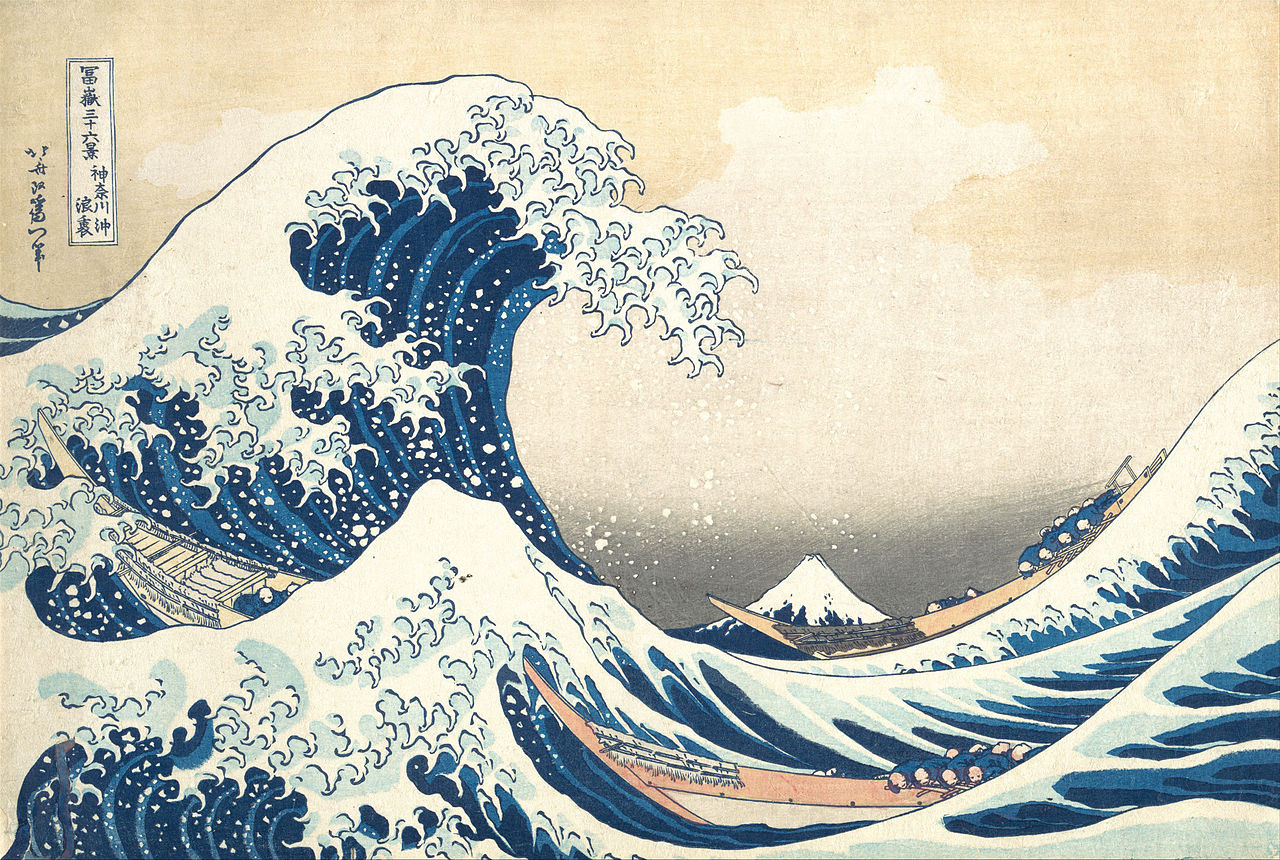
\includegraphics[width=\textwidth]{great_wave}}
        \caption*{\textit{"The Great Wave off Kanagawa"}, Katsushika Hokusai est. 1829}
    \end{figure}
\end{titlepage}

	
\tableofcontents
\pagebreak
   
\section{Introduction}
A tsunami is a single or series of ocean waves which are generated by sudden displacements in the sea floor, landslides, or volcanic activity \cite{zirker}. These potentially catastrophic ocean waves frequently occur in a basin of the Pacfic Ocean known as the "Ring of Fire" for its historically intense volcanic activity \cite{zirker}. Further background into the geological mechanisms resposible for tsunamis can be found in Zirker's (2013) introductory text \textit{The Science of Ocean Waves: Ripples, Tsunamis, and Stormy Seas} \cite{zirker}. An example of tsunami generation can be seen in figure~\ref{fig:tsu_gen}, which was taken from chapter 3 of Marghany's (2018) \textit{Advanced Geoscience Remote Sensing} \cite{marghany}. 

\begin{figure}[h]
    \centering
    \fbox{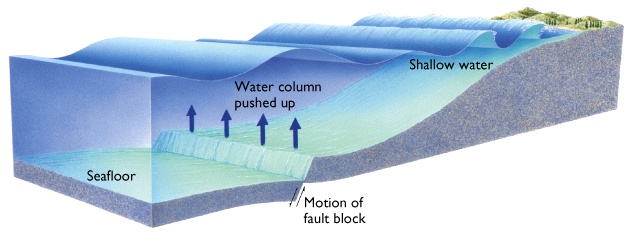
\includegraphics[width=0.75\textwidth]{tsunami_generation}}
    \caption{Tsnumai generation due to horizontal seafloor displacement \cite{marghany}.}
    \label{fig:tsu_gen}
\end{figure}

Transient horizontal displacements resulting from submarine earthquakes and their role in tsunami generation were the focus of  Tanioka' and Satake's (1996) study \textit{Tsunami generation by horizontal displacement of ocean bottom} published in Geophysical Research Letters \cite{satake1}. In this study, they utilize the Satake's (1995) earlier work \textit{Linear and nonlinear computations of the 1992 Nicaragua earthquake tsunami}, which compared and contrasted the success of linear and nonlinear models that governed the generation and propagaion of tsunamis. The linear model utilized in Satake's case study of the Nicaragua earthquake, known as the \textit{shallow-water equations}, and its numerical simulation via a finite-difference method will be the focus of this project.

\section{Shallow-Water Theory}
\textit{Shallow-Water Theory} is the canonical mathematical model for waves propagating non-dispersively in a medium which is much wider than it is deep. The \textit{shallow-water equations} are a system of linear partial-differential equations at the center of Shallow-Water Theory. In this section they will be stated, for a full derivation, see appendix~\ref{a:deriv}. The linear shallow-water equations for a single spatial dimension $x$ and  seafloor shape $H=H(x,y)$ are
\begin{gather}\label{eq:shallow}
    \frac{\partial^2 \eta}{\partial t^2} = \frac{\partial}{\partial x}\left( gH\frac{\partial \eta}{\partial x} \right) + \frac{\partial}{\partial y}\left( gH\frac{\partial \eta}{\partial y} \right)
\end{gather}
where $g$ is gravitational constant and $\eta(x,y,t)$, is the height of the water \cite{salmon}. These equations were taken from chapter 9 of Salmon's (2015) online textbook \textit{Introduction to Ocean Waves}.

\section{The Conservative Form of a Hyperbolic Equation}
\subsection{Introduction}
Before we discuss our process of selection for the scheme used to numerically solve the linear shallow-water equations, it is important to understand the idea of a \textit{conservative form} of a hyperbolic partial-differential equation. First we state the conservative form:
\begin{gather}\label{eq:consv}
	\frac{\partial u}{\partial t} + \nabla \cdot \vec F(u) = 0,
\end{gather}
where $u$ is the \textit{density of the conserved quantity}, and $\vec F (u)$ is the \textit{density flux}. Note that the actual form of $\vec F(u)$ is dependent on the original hyperbolic equation that has been converted into this form. Since $u$ is a density, we will denote its corresponding quantity $\mathbf{u}$ defined by:
\begin{gather}\label{eq:dens}
	\mathbf{u} = \int_V u\hspace*{0.10 cm} dV,
\end{gather}
where $V$ denotes the spatial domain. In physics, a \textit{conservation law} requires that some measurable property of a system does not change with respect to time. For example, the conservation of mass (ignoring energy) requires that any system with perfectly balanced mass transfers, or net-zero mass flux along its boundaries, cannot change its total mass over time. To illustrate the connection between such a conservation law and the conservative form of a hyperbolic equation, we present a short derivation proving the conservation of the quantity $\mathbf{u}$. To start, integrate both sides of the conservative form \ref{eq:consv} term-by-term over the spatial domain $V$:
\begin{gather}\label{eq:int}
	\int_V \frac{\partial u}{\partial t} dV + \int_V \nabla \cdot \vec F(u)\hspace*{0.10 cm} dV = 0.
\end{gather}
Now, we apply Leibniz's rule to change the order of differentiation in the first integral:
\begin{gather}\label{eq:s1}
	\int_V \frac{\partial u}{\partial t} dV = \frac{d}{dt} \int_V u\hspace*{0.10 cm} dV.
\end{gather}
Then, we use the divergence theorem on the second integral, which states that integrating the divergence of the vector field, $\nabla \cdot \vec F(u)$, over the spatial domain $V$ is equal to integrating the vector field over the spatial domain's boundary $A$:
\begin{gather}\label{eq:s2}
	\int_V \nabla\cdot F(u)\hspace*{0.10 cm} dV = \int_A \vec F( u) \cdot \vec n \hspace*{0.10 cm}dA,
\end{gather}
where $\vec n$ is the outward-pointing unit vector along the boundary $A$ (see figure~\ref{fig:domain}). By substituting \ref{eq:s1} and \ref{eq:s2} into \ref{eq:int}, one obtains
\begin{gather}\label{eq:cq}
	\frac{d}{dt} \int_V u \hspace*{0.10 cm} dV =- \int_A \vec F(u) \cdot \vec n \hspace*{0.10 cm}dA.
\end{gather}
Thus, the time derivative of $\mathbf{u}$ (see \ref{eq:dens}) in $V$ is equal to the net flux across the boundary $A$ (the second integral). Note that the unit vectors $\vec n$ are outward-pointing along $A$, meaning that $-\vec n$ must be inward-pointing. Thus, this equation does not necessarily say that $\mathbf{m}$ is conserved: it is a more general statement that $\mathbf{m}$ can only change if there is non-zero net flux along the boundary $A$.
\begin{figure}[h]
	\centering
	\fbox{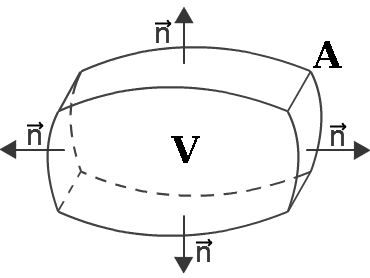
\includegraphics[width=0.50\textwidth]{div}}
	\caption{A spatial domain $\Omega$ and the unit vectors $\vec n$ along its boundary $\partial\Omega$.}
	\label{fig:domain}
\end{figure}

\noindent Now we return to the law of conservation of mass to provide practical intuition regarding \ref{eq:cq}. Assume that the physical system in question is a mass distribution $m$ over some spatial domain $V$, and some mass transfer $\vec F(m)$ within $V$ as well as along $A$. We may state the law of conservation of mass in this case using our previous result \ref{eq:cq}:
\begin{gather}\label{eq:massconsv}
    \frac{d}{dt} \int_V m\hspace*{0.10 cm} dV = - \int_A \vec F(m) \cdot \vec n \hspace*{0.10 cm}dA.
\end{gather}
This offers a clearer picture of the significance of the conserved quantity, as in this case it is the total mass $\mathbf{m}$ of the system:
\begin{gather*}
    \mathbf{m} = \int_V m \hspace*{0.10 cm }dV,
\end{gather*}
In the case where the system is isolated with respect to mass transfers, we know that the flux $A$ is zero everywhere along the boundary:
\begin{gather*}
    \vec F(m) = 0,\quad\text{along } A.
\end{gather*}
This implies that
\begin{gather*}
    \int_A \vec F(m) \cdot \vec n \hspace*{0.10 cm}dA = 0,\quad\text{as } \vec F(m) = 0\text{ along } A.\\
\end{gather*}
Thus, by the statement \ref{eq:massconsv}, we have
\begin{gather*}
    \frac{d}{dt}\int_V m\hspace*{0.10 cm} dV = \frac{d}{dt}\mathbf{m} = 0,
\end{gather*}
that is: the total mass of our system does not change with respect to time. If a system cannot gain or lose mass, the total mass does not change. However, our statement of \ref{eq:massconsv} allows for a more general result: if the net flux along the boundary is zero, we have:
\begin{gather*}
    \int_A \vec F(m) \cdot \vec n \hspace*{0.10 cm}dA = 0.
\end{gather*}
This implies by \ref{eq:massconsv} that the total mass, yet again, cannot change in time. If a system is given some mass but the exactly same amount of mass is removed from the system, the total mass does not change even though the system is not closed with respect to mass transfers along its boundary. Further, if we know the net flux, then we know exactly how the total mass $\mathbf{m}$ will change in time.

\subsection{The Numerical Importance of the Conservative Form}


\subsection{The Conservative Form of The Shallow-Water Equations}


\section{Numerical Methodolgy}
\subsection{A Test Problem}
In this section we derive and evaluate a number of common numerical schemes for the solution of a test problem: the wave equation in two dimensions
\begin{gather}\label{eq:wave}
    \frac{\partial^2 u}{\partial t^2} = c^2\left(\frac{\partial^2 u}{\partial x^2} + \frac{\partial^2 u}{\partial y^2} \right)\qquad\text{for }(x,y)\in\Omega,
\end{gather}
where $c$ denotes the propagation speed, and $\Omega$ denotes the interior of our spatial domain. For this equation, we consider homogenous Dirchlet boundary conditions
\begin{gather}\label{eq:bcs}
    u(t,x,y) = 0\qquad\text{for }(x,y)\in\partial\Omega,
\end{gather}
where $\partial\Omega$ denotes the exterior of our spatial domain. Finally, we also consider some initial condition
\begin{gather}\label{eq:ic}
    u(t,x,y) = f(x,y)\qquad\text{for }t=t_0.
\end{gather}
The equation \ref{eq:shallow}  that we plan to numerically solve is very similar to this equation, as both are linear second-order hyperbolic partial differential equations. Further, we will be using the same boundary and initial conditions. Because of this, we select the scheme that we find to be optimal in terms of both time and accuracy.

\noindent However, we first state \label{eq:wave} in \noindent{conservative form}.

\subsection{Explicit Schemes}
\subsubsection{The Upwind Scheme}


The shallow water equation~\ref{eq:shallow} is a linear, hyperbolic partial differential equation suitable for a two-dimensional discretization in space, numerically solvable via the Leapfrog scheme as presented in chapter 4 of Rezzolla's \textit{Lecture Notes on Numerical Methods for the Solution of Hyperbolic Partial Differential Equations} \cite{rezzolla}: \colorbox{red}{Statement and Scheme Later}.
\subsection{Implicit Schemes}

\subsection{Iterative Schemes}

\section{Application: Fukushima Daiichi Nuclear Disaster}
The shallow water equation requires a choice of a particular seafloor shape $H=H(x,y)$. To test the shallow-water equation, the geography of eastern Japan, specifically $\overline{\text{O}}\text{kuma}$, Fukushima will be used and a tsunami resulting from an earthquake with its epicenter at the same location as the $\text{T}\overline{\text{o}}\text{hoku}$ earthquake will be simulated. If the tsnumai's wave front reaches the Fukushima Daiichi Nuclear Power Plant, it will be demonstrated whether or not the shallow-wave equation is suitable for simulating not only tsunamis, but areas that may be at risk of flooding from tsunamis.

\appendix
\section{Derivation of The Shallow Water Equations}\label{a:deriv}
\colorbox{red}{Later.}
\section{The Leapfrog Method}
\subsection{Stability}
\colorbox{red}{Later.}
\subsection{Consistency}
\colorbox{red}{Later.}
\subsection{Convergence}
\colorbox{red}{Later.}

\begin{thebibliography}{1}
\bibitem{zirker}
Jack B Zirker.
\textit{The Science of Ocean Waves: Ripples, Tsunamis, and Stormy Seas}.
John Hopkins University Press, 22 October 2013. 
Accessed via Arthur Lakes Library at the Colorado School of Mines, March 31, 2018.
    
\bibitem{marghany}
Maged Marghany.
\textit{Simulation of Tsunami Impact on Sea Surface Salinity along Banda Aceh Coastal Waters, Indonesia}.
Advanced Geoscience Remote Sensing, Ch 3. Intech, 2014. Accessed via In Tech Open, March 31, 2018.
    
\bibitem{satake1}
Yuichiro Tanioka, Kenji Satake.
\textit{Tsunami generation by horizontal displacement of ocean bottom}.
Geophysical Research Letters, Vol 3, No 8, 15 April 1996. American Geophysical Union Publications. Accessed via Wiley Online Library, March 31, 2018.

\bibitem{salmon}
Rick Salmon.
\textit{Introduction to Ocean Waves}.
Scripps Institution of Oceanography, University of California, San Diego, 7 December 2015. Accessed via Rick Salmon's website via http://pordlabs.ucsd.edu/rsalmon/, March 31, 2018.

\bibitem{rezzolla}
Luciano Rezzolla.
\textit{Lecture Notes on Numerical Methods for the Solution of Hyperbolic Partial Differential Equations}.
SISSA, International School of Advanced Studies, Trieste, Italy, 2 August 20015. Accessed via Luciano Rezzolla's website via http://www.sissa.it/~rezzolla, March 31, 2018.

\end{thebibliography}
	
\end{document}